Графиком функции такого вида является прямая. 

\begin{figure}[h!]
	\centering
	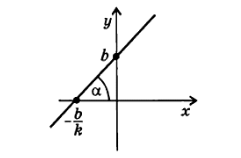
\includegraphics[width=0.4\textwidth]{img/lin.png}
	\caption{Линейная функция}
\end{figure}

Построение делаем с помощью таблицы, достаточно 2 точек (Почему?).

Аналитика параметров функции:

\begin{itemize}
    \item Параметр $b$ - это $f(0) = b$, а значит, точка пересечения с осью OY;
    \item Параметр $k$ - это угловой коэффициент - $k = \tg{\alpha}$ - тангенс угла наклона нашей прямой. Как мы знаем, если $
    \tg{\alpha} > 0 (k > 0)$ то угол $\alpha$ острый, если  $
    \tg{\alpha} < 0 (k < 0)$ то угол $\alpha$ тупой.
\end{itemize}

